\documentclass[aspectratio=169,11pt]{beamer}
\usepackage[T1]{fontenc}
\usepackage{lmodern,amsmath,amssymb,booktabs,graphicx}
\definecolor{ink}{HTML}{17324D}
\definecolor{accent}{HTML}{007C83}
\setbeamercolor{normal text}{fg=ink,bg=white}
\setbeamercolor{structure}{fg=accent}
\setbeamercolor{frametitle}{fg=ink}
\setbeamerfont{frametitle}{series=\bfseries,size=\large}
\setbeamertemplate{navigation symbols}{}
\newcommand{\slidelabel}{\insertframenumber}
\setbeamertemplate{footline}{\hbox to \paperwidth{\hfill\scriptsize ECON 847\quad Yifan and Wenhan\quad\slidelabel\hspace{5mm}}\vskip3mm}
\setbeamersize{text margin left=8mm,text margin right=8mm}
\newcommand{\captiontext}[1]{\par\medskip{\footnotesize\raggedright #1\par}}
\newcommand{\KC}{Kimberly-Clark}
\hypersetup{pdftitle={What would a Scott--Kimberly-Clark merger do to bathroom tissue prices?},pdfauthor={Yifan and Wenhan}}
\begin{document}

% ---------------------------------------------------------------- 1 (Wenhan)
\begin{frame}[plain]
\vspace{12mm}{\LARGE\bfseries What would a Scott--\KC\ merger\\[2mm]do to bathroom tissue prices?}\par
\vspace{8mm}{\large Dominick's scanner data, 1991--1992}\par
\vspace{9mm}Yifan and Wenhan\par ECON 847\quad November 23, 2026
\end{frame}

% ---------------------------------------------------------------- 2 (Wenhan)
\begin{frame}{The merger raises prices; how much depends on substitution within the category}
\begin{itemize}\setlength\itemsep{3.5mm}
\item Put Scott and \KC\ products under one owner. All manufacturers reset prices.
\item Demand, the product set and marginal costs stay fixed. No merger efficiencies.
\item Across our specifications: category prices rise \textbf{0.2--3.4\%}; \KC\ prices rise \textbf{1--24\%}.
\item With price in dollars, the implied cost of Scott single rolls is negative. With log price, costs are sensible and the effects are smaller: \KC\ prices rise \textbf{1--11\%}.
\end{itemize}
\captiontext{The actual merger occurred in 1995. We simulate earlier conditions, not that transaction's remedies or efficiencies.}
\end{frame}

% ---------------------------------------------------------------- 3 (Wenhan)
\begin{frame}{Scott dominates package sales; \KC\ is smaller}
\begin{columns}[T,onlytextwidth]
\column{.58\textwidth}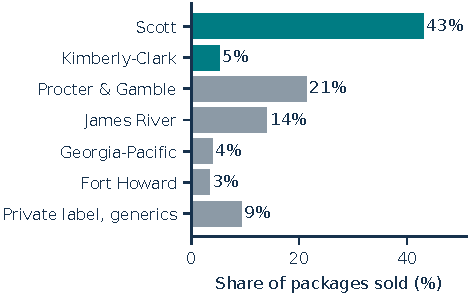
\includegraphics[width=\linewidth]{figures/manufacturers.pdf}
\column{.39\textwidth}\small
\textbf{Scott: 43\%.} ScotTissue and Cottonelle.\par\medskip
\textbf{\KC: 5\%.} Kleenex and Delsey. Kleenex Bath Tissue rolled out in selected regions in 1991.\par\medskip
\KC's small share is why its own prices can rise a lot while the category average rises little.
\end{columns}
\captiontext{Shares of packages sold at Dominick's, 1991--1992.}
\end{frame}

% ---------------------------------------------------------------- 4 (Wenhan)
\begin{frame}{Within a store and UPC, prices move through temporary price cuts}
\begin{columns}[T,onlytextwidth]
\column{.59\textwidth}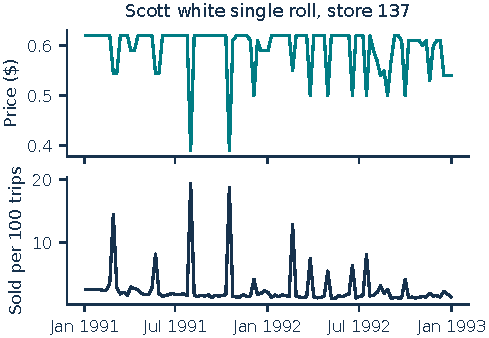
\includegraphics[width=\linewidth]{figures/promotions.pdf}
\column{.38\textwidth}\small
\textbf{98.1\%} of price variance is across store--UPC averages. Most of that is pack size: a 12-pack costs more than a single roll. Differences between stores are 0.2\%.\par\medskip
\textbf{1.9\%} is within a store and UPC over time.\par\medskip
After fixed effects, the price coefficient is identified from these week-to-week price changes within a store and UPC. They are mostly temporary price cuts.
\end{columns}
\end{frame}

% ---------------------------------------------------------------- 5 (Wenhan)
\begin{frame}{A market is a store-week; a product is a UPC}
\begin{columns}[T,onlytextwidth]
\column{.47\textwidth}\small
\begin{tabular}{@{}lr@{}}\toprule
Store-weeks & 7,996\\
Stores / UPCs & 83 / 50\\
Median UPCs per market & 32\\
Median package price & \$1.15\\
Single rolls, share of packages sold & 37.7\%\\
Median outside share & 86.7\%\\\bottomrule
\end{tabular}
\column{.50\textwidth}\small
\textbf{Market:} store-week. Averaging over weeks would remove the temporary price cuts.\par\medskip
\textbf{Product:} UPC. This keeps brand, pack size and variant.\par\medskip
\textbf{Share:} packages sold divided by shopping trips. \textbf{Outside option:} a trip with no tissue purchase.\par\medskip
\textbf{Dropped:} products with no sales in the week; store-weeks without seven days of traffic counts or with a missing instrument.
\end{columns}
\captiontext{259,986 observations; 94\% of packages sold in 1991--1992.}
\end{frame}

% ---------------------------------------------------------------- 6 (Wenhan)
\begin{frame}{Logit demand, estimated by 2SLS with one price instrument}
\vspace{-2mm}
\[
\log\frac{s_{jt}}{s_{0t}}=\alpha_{j,\mathrm{store}}+\tau_t+\beta f(p_{jt})+\gamma\,\mathrm{Deal}_{jt}+\xi_{jt},
\qquad f(p)=p\ \text{or}\ \log p .
\]
\vspace{-3mm}
\begin{columns}[T,onlytextwidth]
\column{.43\textwidth}\footnotesize
Store--UPC effects $\alpha$ and week effects $\tau$.\par\smallskip
$\xi$: local demand shocks and unrecorded promotions. 12.5\% of packages sell more than 5\% below the usual price with no deal flag.\par\smallskip
The deal dummy is treated as exogenous.
\column{.55\textwidth}\footnotesize\setlength\tabcolsep{4.5pt}
\begin{tabular}{@{}lrrrr@{}}\toprule
First stage & $\hat\pi$ & SE & Partial $R^2$ & $F$\\\midrule
Dollars / AAC & .394 & .039 & .125 & 101\\
Dollars / other zone & 1.052 & .029 & .693 & 1,316\\
Log / AAC & .318 & .048 & .111 & 45\\
Log / other zone & 1.022 & .018 & .788 & 3,246\\\bottomrule
\end{tabular}
\end{columns}
\medskip\footnotesize
\textbf{AAC:} the wholesale cost moves the retail price and is unrelated to this week's demand shock in this store.\par\smallskip
\textbf{Other-zone price:} the same UPC's price in Dominick's other pricing zones moves with common costs and is unrelated to this store's demand shock.\par\smallskip
\textbf{Weakness of both:} promotions are planned by the chain and funded by manufacturers, so they move the instrument and demand together.
\captiontext{$\hat\pi$: coefficient on the instrument. The instrument is in logs when price is in logs.}
\end{frame}

% ---------------------------------------------------------------- 7 (Wenhan)
\begin{frame}{Single rolls: elasticity \texorpdfstring{$\mathbf{-1.0}$}{-1.0} with price in dollars, \texorpdfstring{$\mathbf{-5.2}$}{-5.2} with log price}
\small
\begin{center}\begin{tabular}{lrrr}\toprule
Price / instrument & Price coefficient & SE & Median own elasticity\\\midrule
Dollars / AAC & $-2.028$ & .319 & $-2.326$\\
Dollars / other zone & $-2.689$ & .164 & $-3.084$\\
Log / AAC & $-5.388$ & .558 & $-5.376$\\
Log / other zone & $-5.184$ & .209 & $-5.173$\\\bottomrule
\end{tabular}\end{center}
\begin{center}\begin{tabular}{lrrr}\toprule
Own elasticity by pack size (AAC) & Mean price & Price in dollars & Log price\\\midrule
One roll & \$0.51 & $-1.00$ & $-5.18$\\
Four rolls & \$1.04 & $-2.04$ & $-5.21$\\
Six or more rolls & \$2.85 & $-5.77$ & $-5.37$\\\bottomrule
\end{tabular}\end{center}
\captiontext{Coefficient units differ by price form.}
\end{frame}

% ---------------------------------------------------------------- 8 (Yifan)
\begin{frame}{Nested logit lets tissue products be closer substitutes for each other}
\vspace{-1mm}
\[
\log\frac{s_{jt}}{s_{0t}}=\alpha_{j,\mathrm{store}}+\tau_t+\beta f(p_{jt})+\gamma\,\mathrm{Deal}_{jt}
+\rho\log\frac{s_{jt}}{S_t}+\xi_{jt}
\]
\small $S_t$ is the total share of all tissue products in the market, so $s_{jt}/S_t$ is the product's share of tissue sales.
\begin{itemize}\setlength\itemsep{2.2mm}
\item One nest holds all tissue products. The outside option is alone in its own nest.
\item $\rho=0$ is the plain logit. As $\rho$ rises, a buyer who leaves one tissue product is more likely to pick another tissue product and less likely to buy nothing.
\item $\rho$ is not estimated. $\log(s_{jt}/S_t)$ is endogenous, so estimating $\rho$ needs a second instrument that moves a product's share of tissue sales without moving its demand shock. We have one instrument.
\item We set $\rho$ to 0, 0.25, 0.5 and 0.75, and estimate $\beta$ at each value.
\end{itemize}
\captiontext{$\rho$ here is $1-\lambda$ in the lecture's notation.}
\end{frame}

% ---------------------------------------------------------------- 9 (Yifan)
\begin{frame}{Nesting leaves own-price elasticities alone and changes where lost buyers go}
\footnotesize
\begin{center}\begin{tabular}{@{}r rrr @{\hspace{5mm}} rrr @{\hspace{5mm}} r@{}}\toprule
& \multicolumn{3}{c}{Price in dollars}& \multicolumn{3}{c}{Log price} & Diversion,\\
\cmidrule(r{5mm}){2-4}\cmidrule(r{5mm}){5-7}
$\rho$ & $\hat\beta$ (SE) & Own & Category & $\hat\beta$ (SE) & Own & Category & K--C to Scott\\\midrule
0 & $-2.03$ (0.32) & $-2.33$ & $-1.87$ & $-5.39$ (0.56) & $-5.38$ & $-4.67$ & 5\%\\
0.25 & $-1.53$ (0.24) & $-2.32$ & $-1.41$ & $-4.07$ (0.42) & $-5.39$ & $-3.53$ & 13\%\\
0.50 & $-1.02$ (0.16) & $-2.32$ & $-0.95$ & $-2.75$ (0.28) & $-5.45$ & $-2.38$ & 21\%\\
0.75 & $-0.52$ (0.08) & $-2.35$ & $-0.48$ & $-1.43$ (0.14) & $-5.64$ & $-1.24$ & 29\%\\\bottomrule
\end{tabular}\end{center}
\small
\begin{itemize}\setlength\itemsep{2.5mm}
\item The data fix the own-price elasticity for every $\rho$: about $-2.3$ with price in dollars and $-5.4$ with log price. $\rho$ decides how the lost buyers split between other tissue and the outside option.
\item Diversion is the share of buyers leaving a \KC\ product who switch to a Scott product. It is what the merger internalizes. It depends only on shares and $\rho$.
\end{itemize}
\captiontext{AAC instrument. Own and Category are median own-price and category elasticities.}
\end{frame}

% ---------------------------------------------------------------- 10 (Yifan)
\begin{frame}{Each manufacturer sets prices for all its products; cost is price minus markup}
\small
\[
p=c-(\Omega\odot D)^{-1}s
\qquad\Longrightarrow\qquad
\text{markup }\mu=-(\Omega\odot D)^{-1}s .
\]
$\Omega$: 1 when two products have the same owner. $D$: derivatives of shares with respect to prices.\par\smallskip
Plain logit with price in dollars: $\displaystyle\mu_f=\frac{1}{|\beta|\,(1-S_f)}$, where $S_f$ is the firm's total market share.
\begin{itemize}\setlength\itemsep{2mm}
\item Retail price = wholesale price + the retailer's margin. The retailer's margin is a fixed dollar amount per package.
\item AAC is our measure of the wholesale price. \textbf{Implied manufacturer cost = AAC $-$ $\mu$.}
\item Marginal cost is constant in quantity. We do not estimate a cost function. Cost is the residual, one number per product, store and week.
\item The merger changes $\Omega$ and nothing else.
\end{itemize}
\end{frame}

% ---------------------------------------------------------------- 11 (Yifan)
\begin{frame}{For a Scott single roll, the implied markup is larger than the wholesale price}
\small
With price in dollars, the logit gives every product nearly the same dollar markup: about $1/|\beta|=\$0.49$. A 52-cent roll with a 48-cent wholesale price cannot carry a 49-cent markup, so its implied cost is below zero. With log price, the markup is the same percentage of price for every product, about 19\%, so the problem goes away.\par
\medskip
\begin{columns}[c,onlytextwidth]
\column{.46\textwidth}\small
\begin{tabular}{@{}lr@{}}\toprule
\multicolumn{2}{@{}l}{Scott white single roll}\\\midrule
Retail price & \$0.52\\
Wholesale price (AAC) & \$0.48\\
Markup at $\rho=0$ & \$0.58\\
Markup at $\rho=0.75$ & \$1.01\\
Implied cost & $-\$0.10$ to $-\$0.54$\\\bottomrule
\end{tabular}
\column{.52\textwidth}\centering
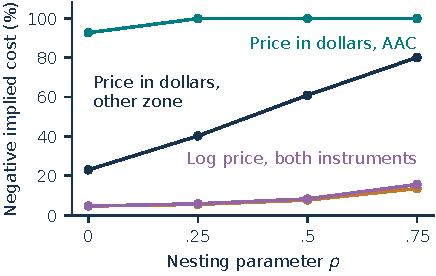
\includegraphics[width=\linewidth]{figures/cost_failures.pdf}
\end{columns}
\captiontext{Chart: share of Scott single-roll packages with negative implied cost.}
\end{frame}

% ---------------------------------------------------------------- 12 (Yifan)
\begin{frame}{Merger: \KC's prices rise most, and more as \texorpdfstring{$\rho$}{rho} rises}
\begin{columns}[T,onlytextwidth]
\column{.40\textwidth}\footnotesize
\textbf{Changes:} ownership. Scott and \KC\ products get one owner.\par\medskip
\textbf{Re-solved:} prices of the six manufacturers' products, and all shares.\par\medskip
\textbf{Held fixed:} marginal costs, non-price utility (fixed effects, deal flags, demand shocks), market size, the product set, the retailer's dollar margin, private-label prices.\par\medskip
\textbf{Algorithm:} start from observed prices and repeat
$p\leftarrow\tfrac12\,p+\tfrac12\,\bigl(c+\mu(p)\bigr)$
until prices stop moving.
\column{.58\textwidth}\centering
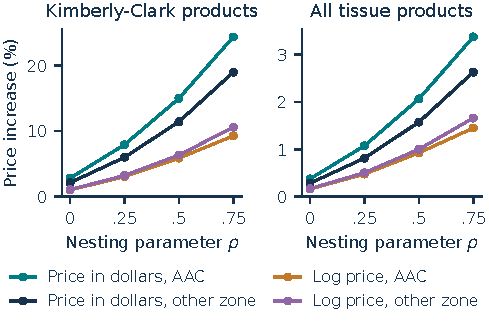
\includegraphics[width=\linewidth]{figures/price_sensitivity.pdf}
\end{columns}
\medskip\small
\KC\ prices: \textbf{+1\% to +11\%} with log price, \textbf{+2\% to +24\%} with price in dollars. Scott: +0.3\% to +4.8\%. Category: +0.2\% to +3.4\%.
\captiontext{Percent, weighted by packages sold. 7,960 of 7,996 store-weeks.}
\end{frame}

% ---------------------------------------------------------------- 13 (Yifan)
\begin{frame}{What we conclude}
\begin{itemize}\setlength\itemsep{4mm}
\item The merger raises prices. \KC's prices rise most. Category prices rise little, because \KC\ sells 5\% of packages.
\item The log-price model gives sensible costs: implied cost is non-negative for 93\% to 98\% of packages. In it the merger raises \KC\ prices by \textbf{1\% to 11\%} and category prices by \textbf{0.2\% to 1.7\%}, depending on $\rho$.
\item The dollar-price model predicts larger effects, and those come from markups that are too large to be real.
\item The range that remains comes from $\rho$. Estimating it needs a second instrument.
\end{itemize}
\end{frame}

% ---------------------------------------------------------------- Backup
\appendix
\renewcommand{\slidelabel}{Backup B\the\numexpr\value{framenumber}-13\relax}

\begin{frame}{A typical market: many products, each with a small share}
\centering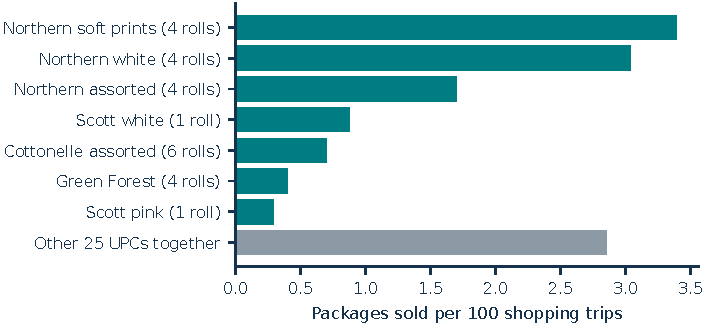
\includegraphics[width=.84\textwidth]{figures/typical_market.pdf}
\captiontext{Store 72, week of May 2, 1991: 32 UPCs on sale; 86.7\% of shopping trips bought no tissue.}
\end{frame}

\begin{frame}{One store-week sold as many packages as it had shopping trips}
\begin{columns}[T,onlytextwidth]
\column{.44\textwidth}
\begin{tabular}{@{}lr@{}}\toprule
\multicolumn{2}{@{}l}{Store 124, week of October 17, 1991}\\\midrule
Shopping trips & 29,213\\
Tissue packages sold & 29,209\\
of which Scott & 28,023\\
Scott single rolls at \$0.39 & 27,916\\\bottomrule
\end{tabular}
\column{.52\textwidth}
Our share is packages sold divided by shopping trips. Here it is 99.99\%.\par\medskip
The model reads this as almost every shopper buying exactly one package. More likely, fewer shoppers bought several 39-cent rolls each.\par\medskip
A one-package-per-trip model does not describe weeks like this one.
\end{columns}
\end{frame}

\begin{frame}{The retailer margin rule changes the merger effects little}
\small\begin{center}\begin{tabular}{lrrrr}\toprule
&\multicolumn{2}{c}{Dollar margin}&\multicolumn{2}{c}{Percentage margin}\\
\cmidrule(lr){2-3}\cmidrule(lr){4-5}
Price / instrument&Category&K--C&Category&K--C\\\midrule
Dollars / AAC & 0.38 & 2.82 & 0.37 & 3.12\\
Dollars / other zone & 0.28 & 2.13 & 0.28 & 2.36\\
Log / AAC & 0.16 & 1.03 & 0.16 & 1.13\\
Log / other zone & 0.17 & 1.08 & 0.16 & 1.18\\\bottomrule
\end{tabular}\end{center}
\normalsize
\textbf{Dollar margin:} retail price = wholesale price + a fixed dollar amount.\par\smallskip
\textbf{Percentage margin:} the retailer keeps a fixed share $m_j$ of the retail price, so the wholesale price is $(1-m_j)\,p_j$ and implied cost is $(1-m_j)\,p_j-\mu_j$.
\captiontext{Price increases in percent at $\rho=0$, weighted by packages sold. 7,960 of 7,996 store-weeks.}
\end{frame}

\begin{frame}{Mixed logit: we tried it and it failed its specification test}
\begin{itemize}\setlength\itemsep{3.5mm}
\item Eight mixed-logit specifications estimated with PyBLP. Six converged.
\item The price coefficient varies with store demographics: household size or income.
\item Instruments: AAC or other-zone price. Samples: all pack sizes, or multipacks only.
\item Five of the six converged specifications reject the joint test of their moment conditions.
\item We therefore use the logit and nested logit, where each assumption is visible.
\end{itemize}
\end{frame}

\begin{frame}{Consumer surplus falls by 0.03 to 0.34 cents per shopping trip}
\small
\[
\Delta CS=\frac{\log\bigl(1+e^{L^{\mathrm{post}}/h}\bigr)-\log\bigl(1+e^{L^{\mathrm{pre}}/h}\bigr)}{|\beta|},
\qquad L=\log\sum_j e^{h\delta_j},\qquad h=\frac{1}{1-\rho}.
\]
\begin{center}\begin{tabular}{lrrrr}\toprule
&\multicolumn{2}{c}{$\rho=0$}&\multicolumn{2}{c}{$\rho=0.75$}\\
\cmidrule(lr){2-3}\cmidrule(lr){4-5}
Instrument & Cents per trip & Total & Cents per trip & Total\\\midrule
AAC & 0.04 & \$66 thousand & 0.34 & \$528 thousand\\
Other zone & 0.03 & \$49 thousand & 0.27 & \$411 thousand\\\bottomrule
\end{tabular}\end{center}
\captiontext{Loss in consumer surplus, price in dollars. Totals are over two years in 83 stores.}
\end{frame}
\end{document}
